% !TeX root = ..\main.tex
\section{Kiến trúc hệ thống}
\subsection{Tổng quan}
\begin{figure}[!htp]
	\centering
	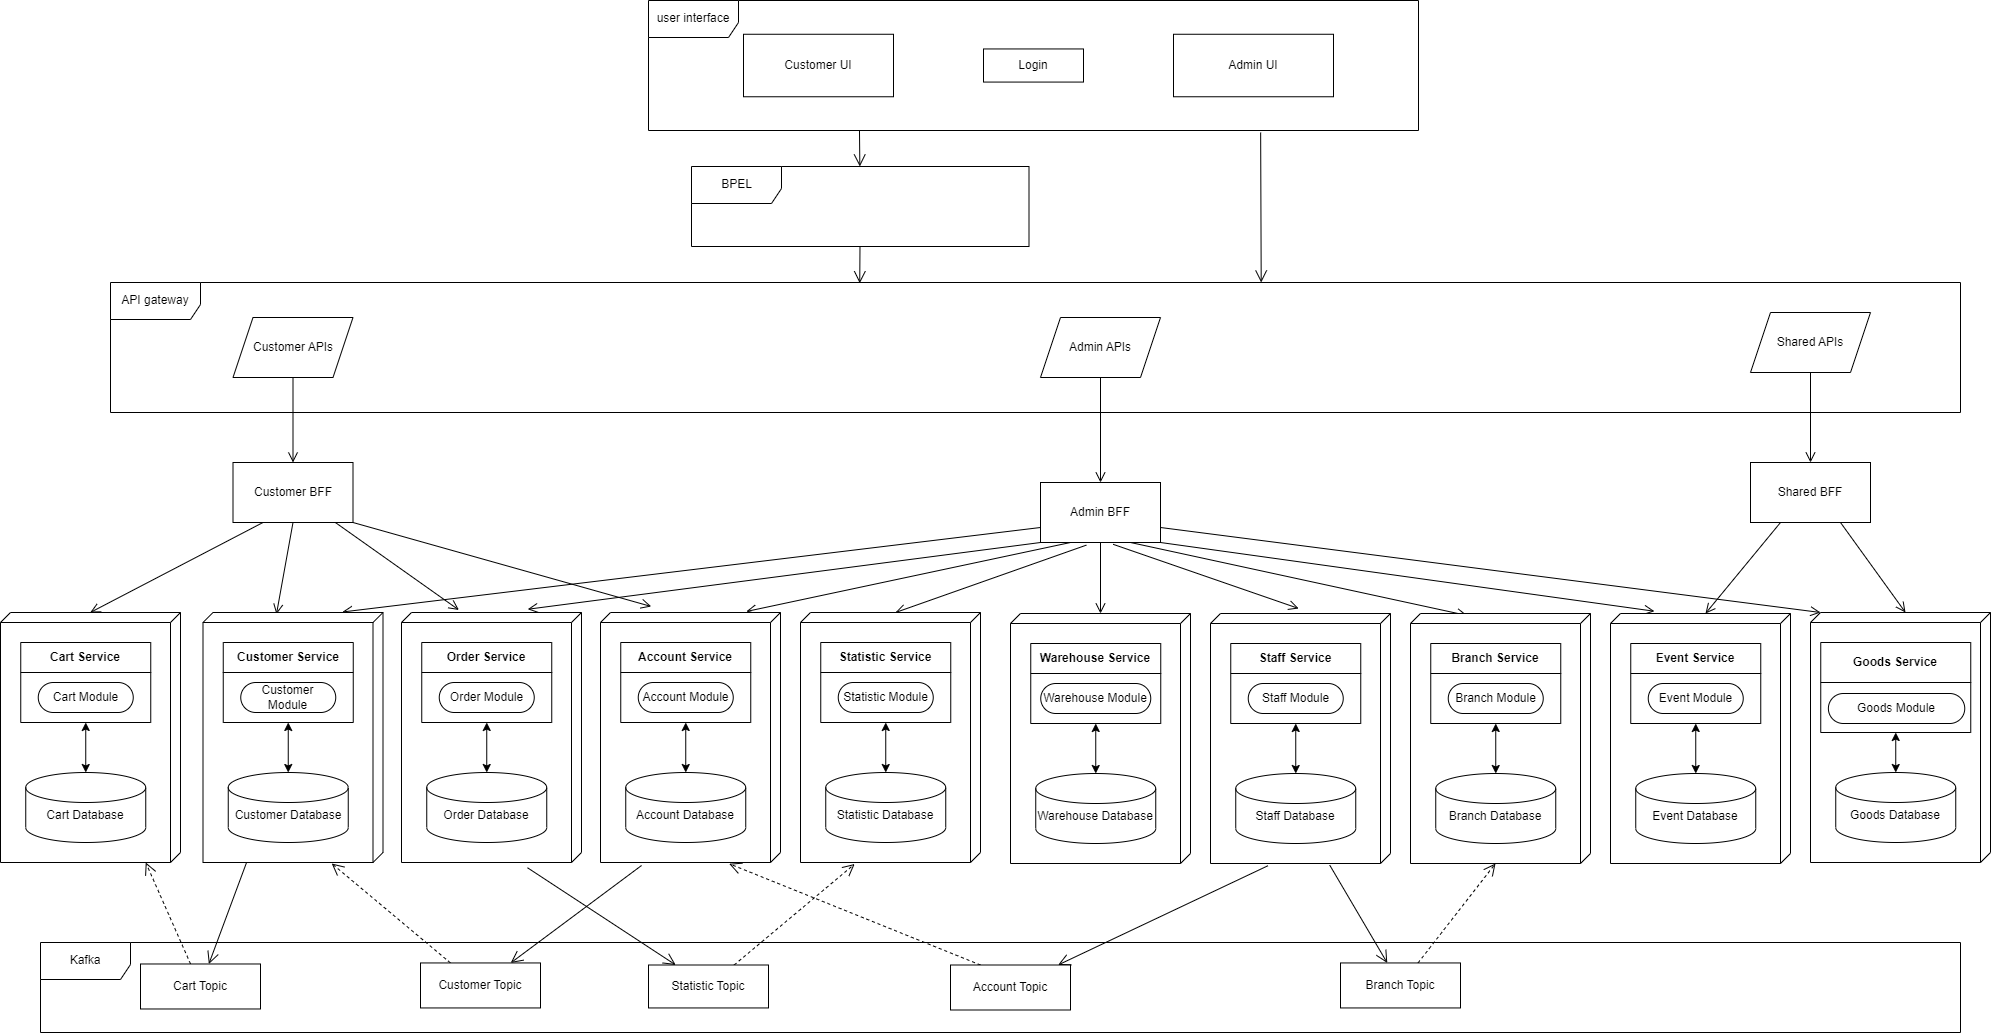
\includegraphics[width=6in]{img/Architecture/general-architect.png}
	\newline
	\caption{Tổng quan kiến trúc hệ thống}
\end{figure}

\subsection{Tầng UI}




\subsubsection{CustomerUI}
Module này bao gồm các class dùng để hiển thị UI đối với phía khách hàng
\begin{figure}[!htp]
	\centering
	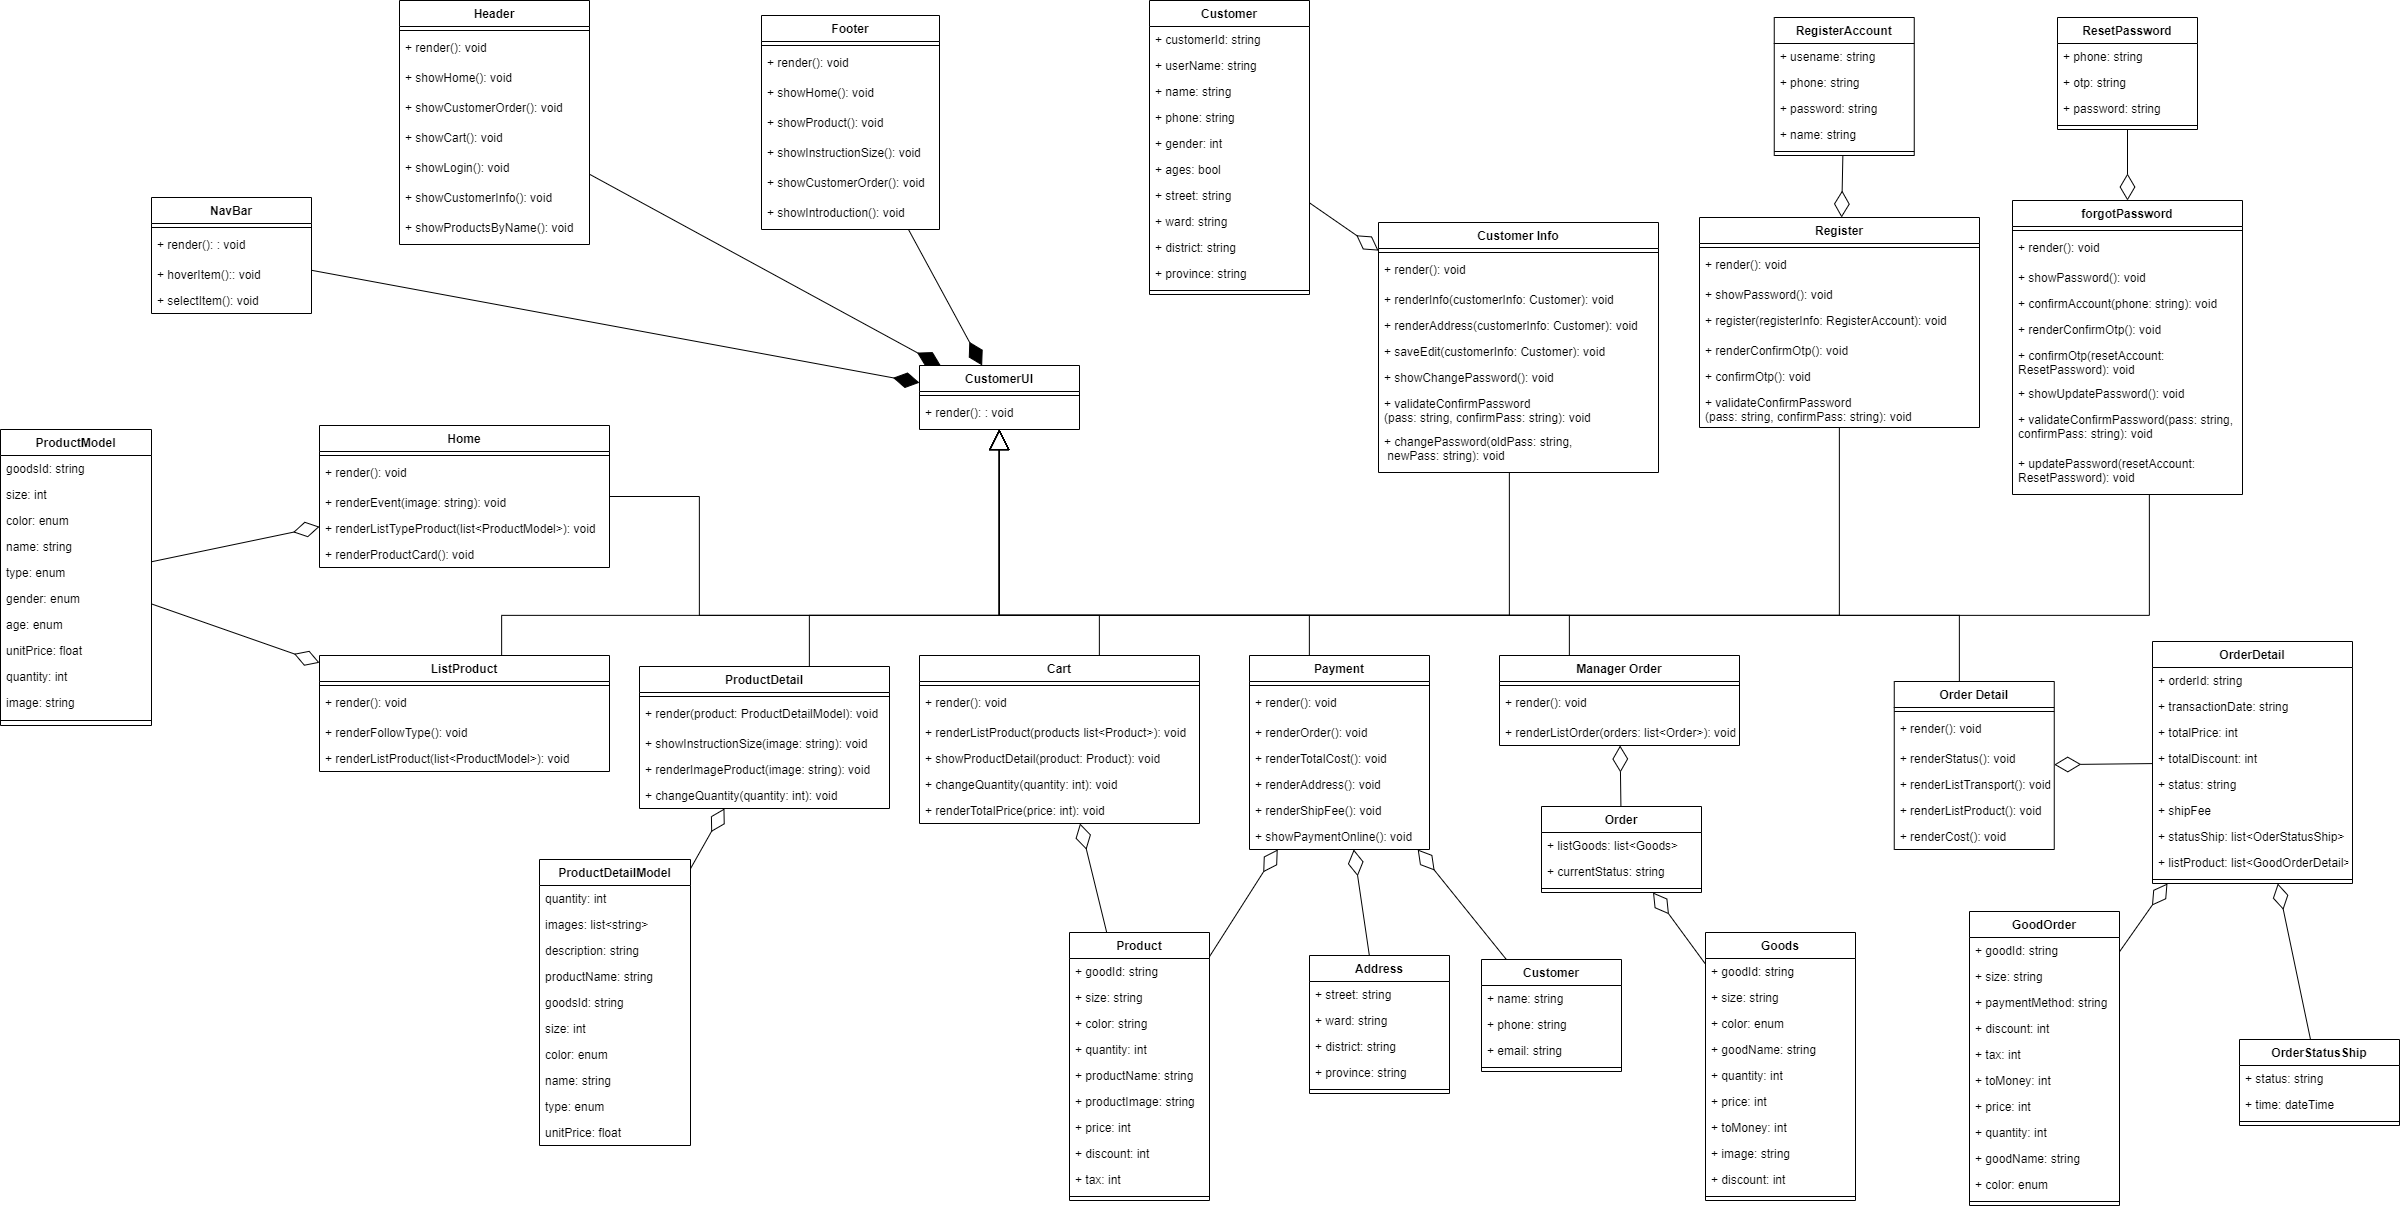
\includegraphics[width=17cm]{img/Architecture/UI/customer UI.png}
	\newline
	\caption{Lược đồ class của Module CustomerUI}
\end{figure}
\textbf{Mô tả:}
\begin{quote}
	\begin{itemize}
		\item CustomerUI
		\item NavBar
		\item Header
		\item Footer
		\item ..
	\end{itemize}
\end{quote}

\subsubsection{LoginUI}
LoginUI là một class dùng để hiển thị trang đăng nhập cho cả phía khách hàng và quản trị viên
\begin{figure}[!htp]
	\centering
	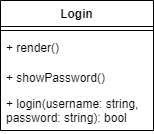
\includegraphics[width=2cm]{img/Architecture/UI/loginUI.png}
	\newline
	\caption{Lược đồ class của LoginUI}
\end{figure}
\textbf{Mô tả:}
\begin{quote}
	\begin{itemize}
		\item CustomerUI
		\item NavBar
		\item Header
		\item Footer
		\item ..
	\end{itemize}
\end{quote}

\subsubsection{AdminUI}
Module này bao gồm các class dùng để hiển thị UI đối với phía quản trị viên

\begin{figure}[!htp]
	\centering
	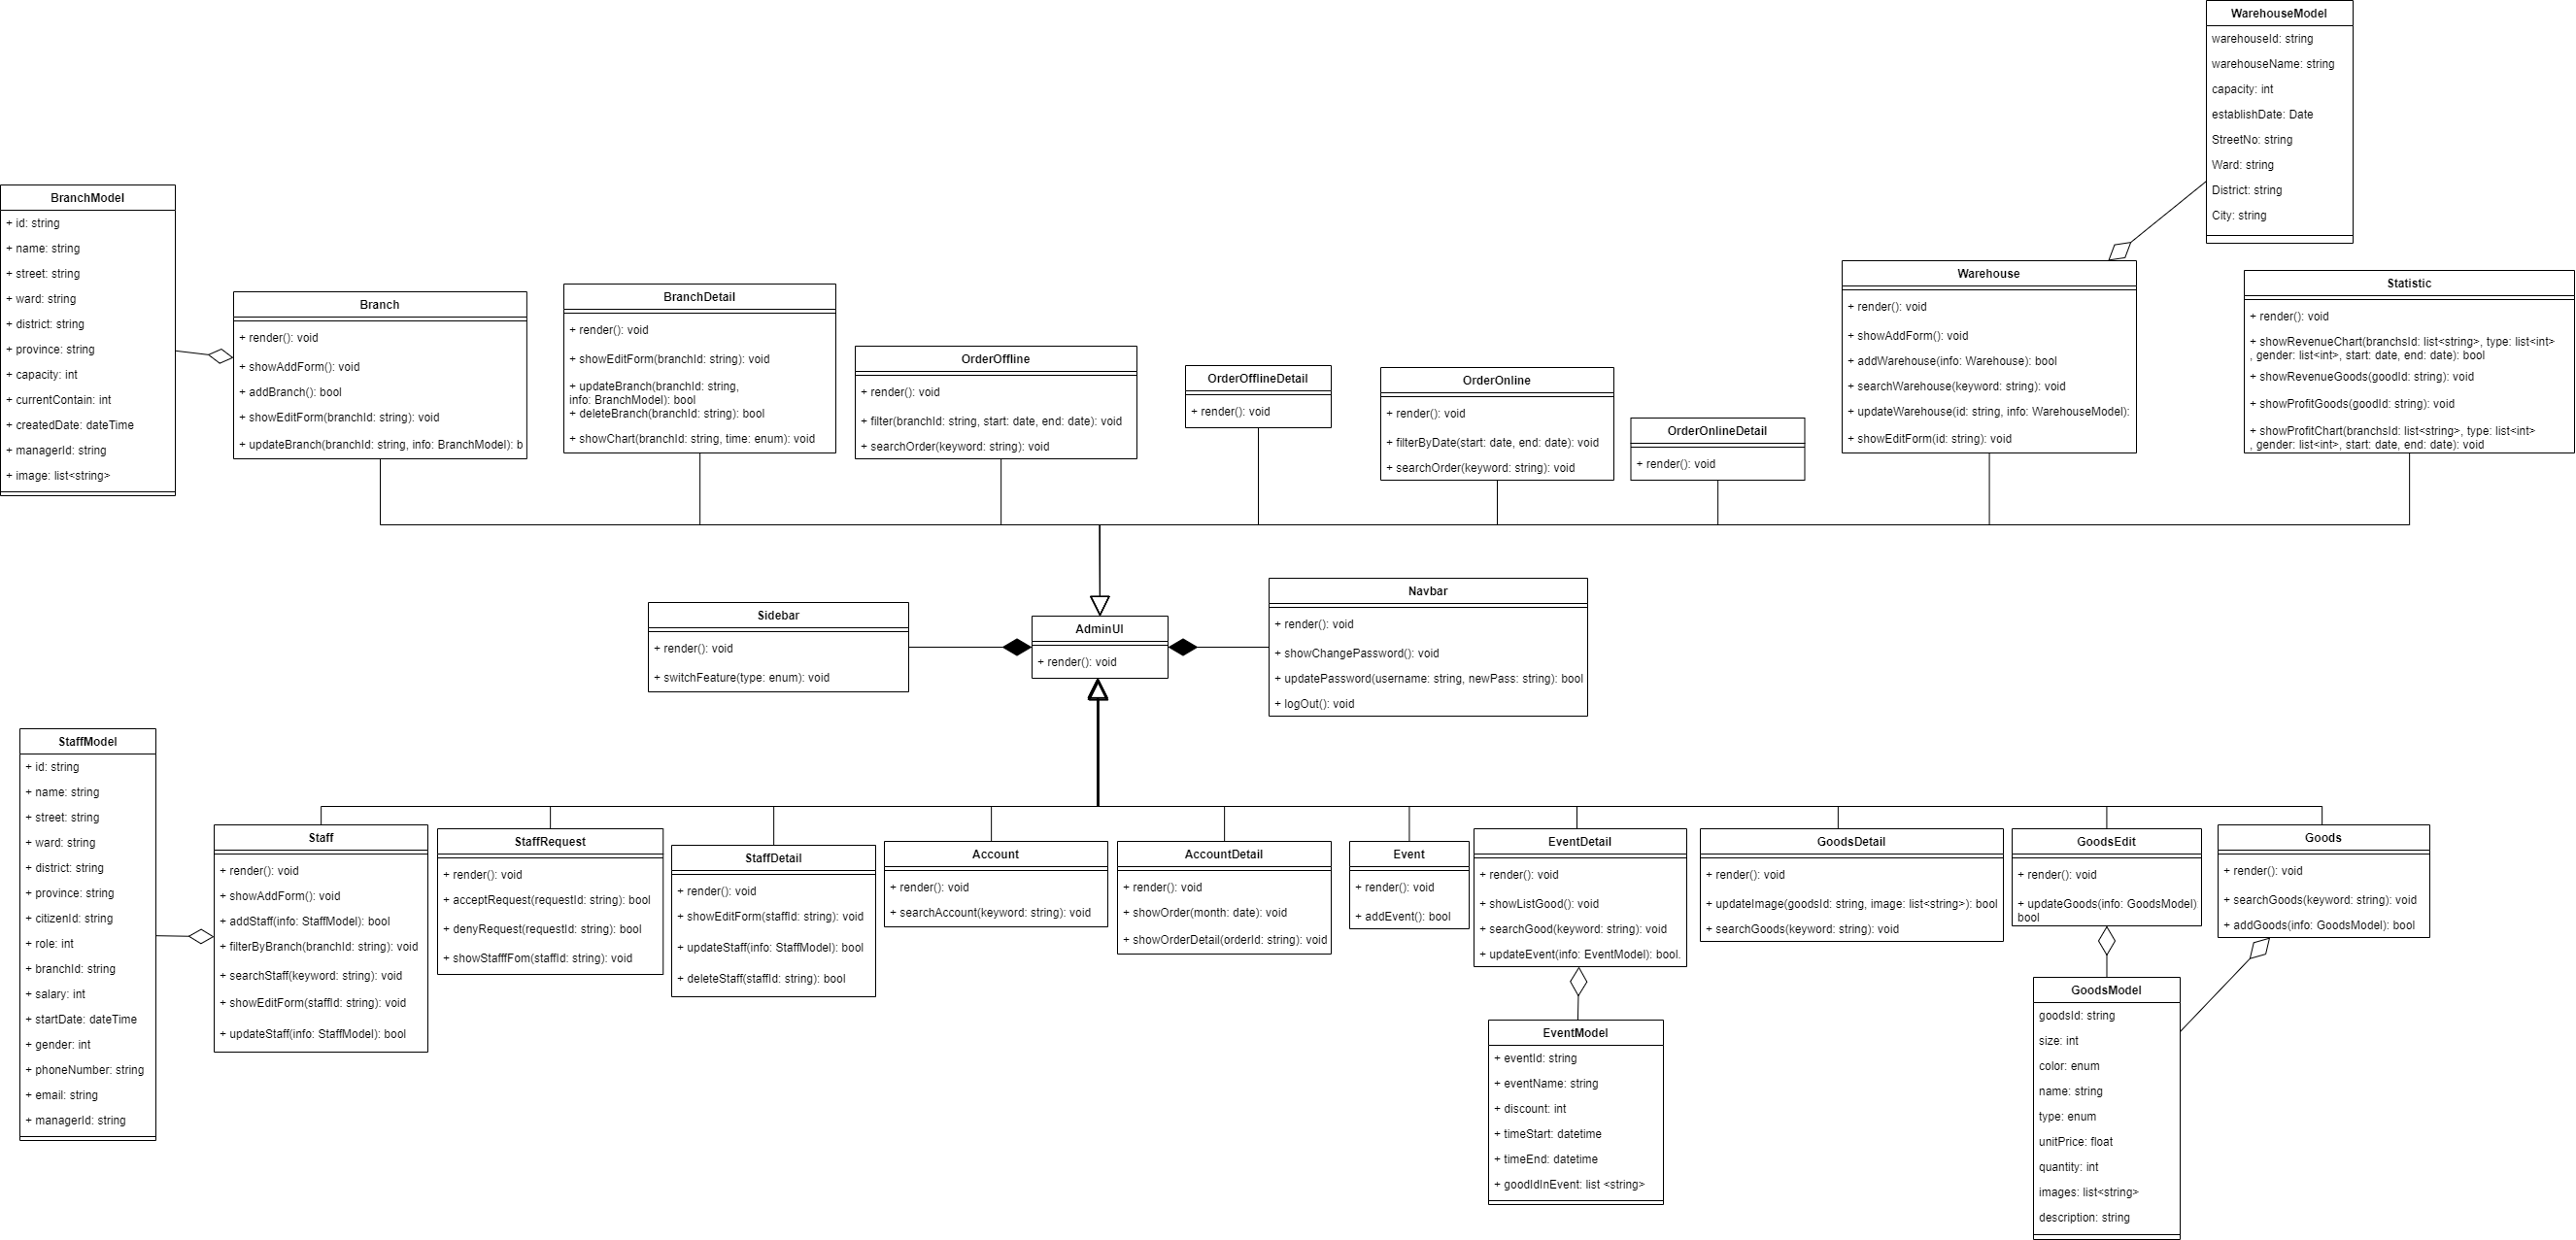
\includegraphics[width=17cm]{img/Architecture/UI/adminUI.png}
	\newline
	\caption{Lược đồ class của Module AdminUI}
\end{figure}
\textbf{Mô tả:}
\begin{quote}
	\begin{itemize}
		\item CustomerUI
		\item NavBar
		\item Header
		\item Footer
		\item ..
	\end{itemize}
\end{quote}





\subsection{Tầng API}
\subsubsection{Customer APIs}
Module này dùng để chứa các API được xuất ra ngoài cho phía khách hàng

\subsubsection{Admin APIs}
Module này dùng để chứa các API được xuất ra ngoài cho phía quản trị viên

\subsubsection{Shared APIs}
Module này dùng để chứa các API được xuất ra ngoài cho bất kì đối tượng người dùng nào




\subsection{Tầng service}

Lược đồ class ở tậng service được xây dựng theo các thành phần sau:
\begin{itemize}
	\item Repository: Class dùng để truy cập trực tiếp đến dữ liệu trong Database
	\item Model: Class dùng để chứa thông tin nhận lên từ Database
	\item Controllers: Class dùng để xử lý các logic nghiệp vụ
	\item Response: Class chứa thông tin trả về khi có yêu cầu từ bên ngoài
	\item Các Interface: Giúp đảm bảo nguyên lý \textbf{Dependency inversion principle} của \textbf{SOLID}
	      \begin {itemize}
	\item IRepository: Cung cấp các api cho các class Controller
	\item IController: Cung cấp các api để bên ngoài service truy cập đến
\end{itemize}
\end{itemize}



\subsubsection{Customer Order Service}
\begin{figure}[!htp]
	\centering
	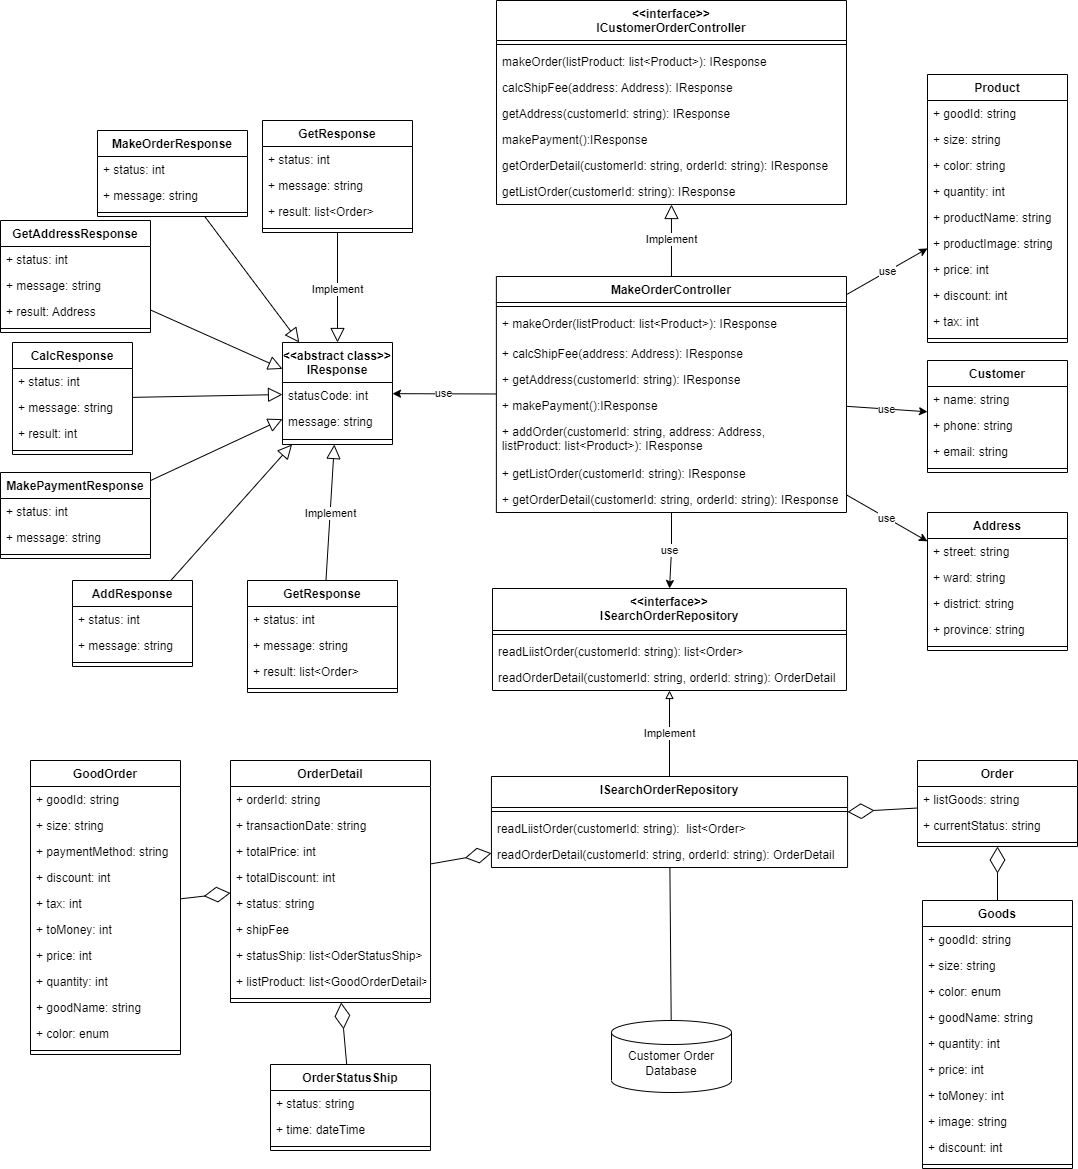
\includegraphics[width=13cm]{img/Architecture/service/CustomerOrderService.png}
	\newline
	\caption{Lược đồ class của Customer Order Service}
\end{figure}



\subsubsection{Cart Service}
\begin{figure}[!htp]
	\centering
	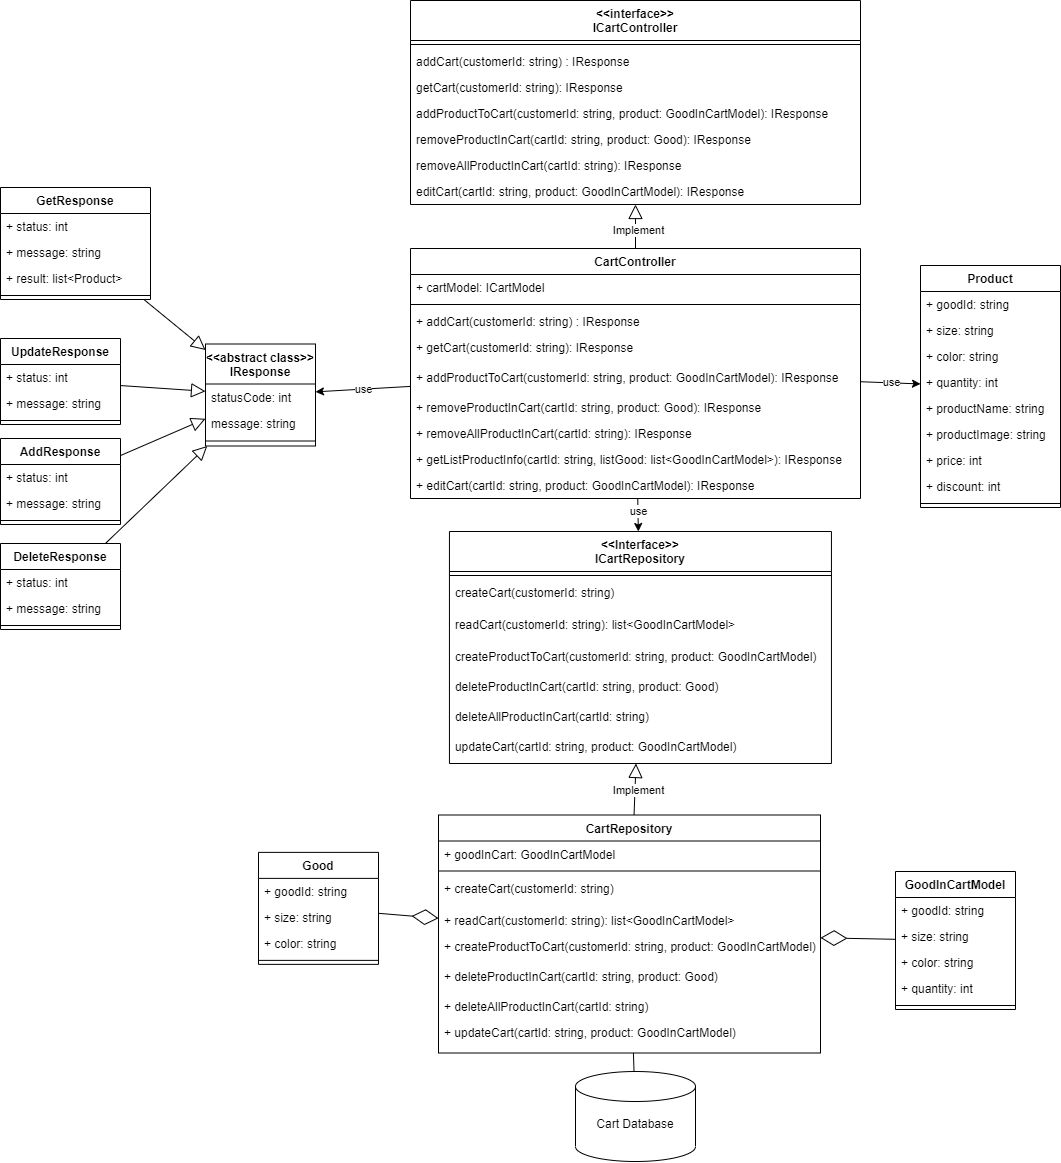
\includegraphics[width=11cm]{img/Architecture/service/CartService.png}
	\newline
	\caption{Lược đồ class của Cart Service}
\end{figure}


\subsubsection{Customer Service}
\begin{figure}[!htp]
	\centering
	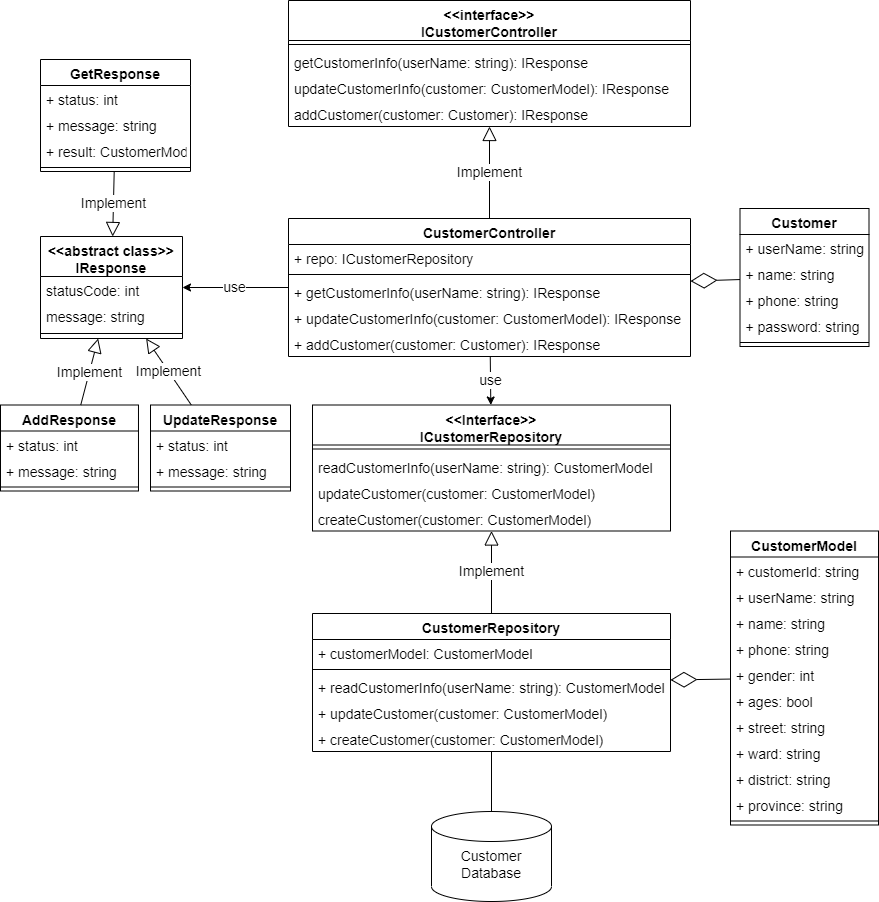
\includegraphics[width=11cm]{img/Architecture/service/CustomerService.png}
	\newline
	\caption{Lược đồ class của Customer Service}
\end{figure}



\subsubsection{Order Service}
\begin{figure}[!htp]
	\centering
	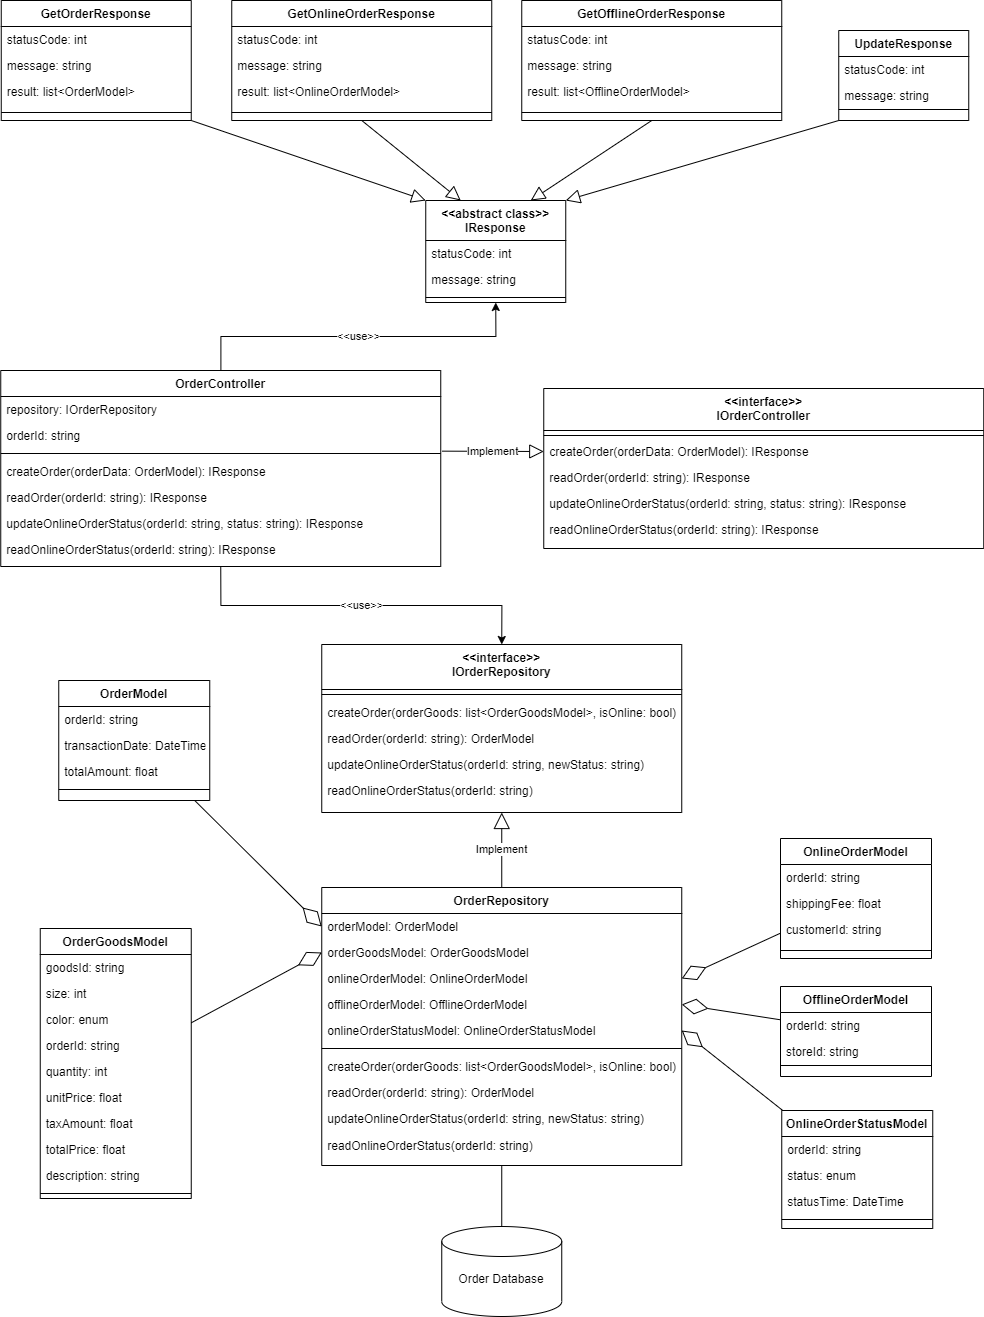
\includegraphics[width=11cm]{img/Architecture/service/OrderService.png}
	\newline
	\caption{Lược đồ class của Order Service}
\end{figure}



\subsubsection{Account Service}
\begin{figure}[!htp]
	\centering
	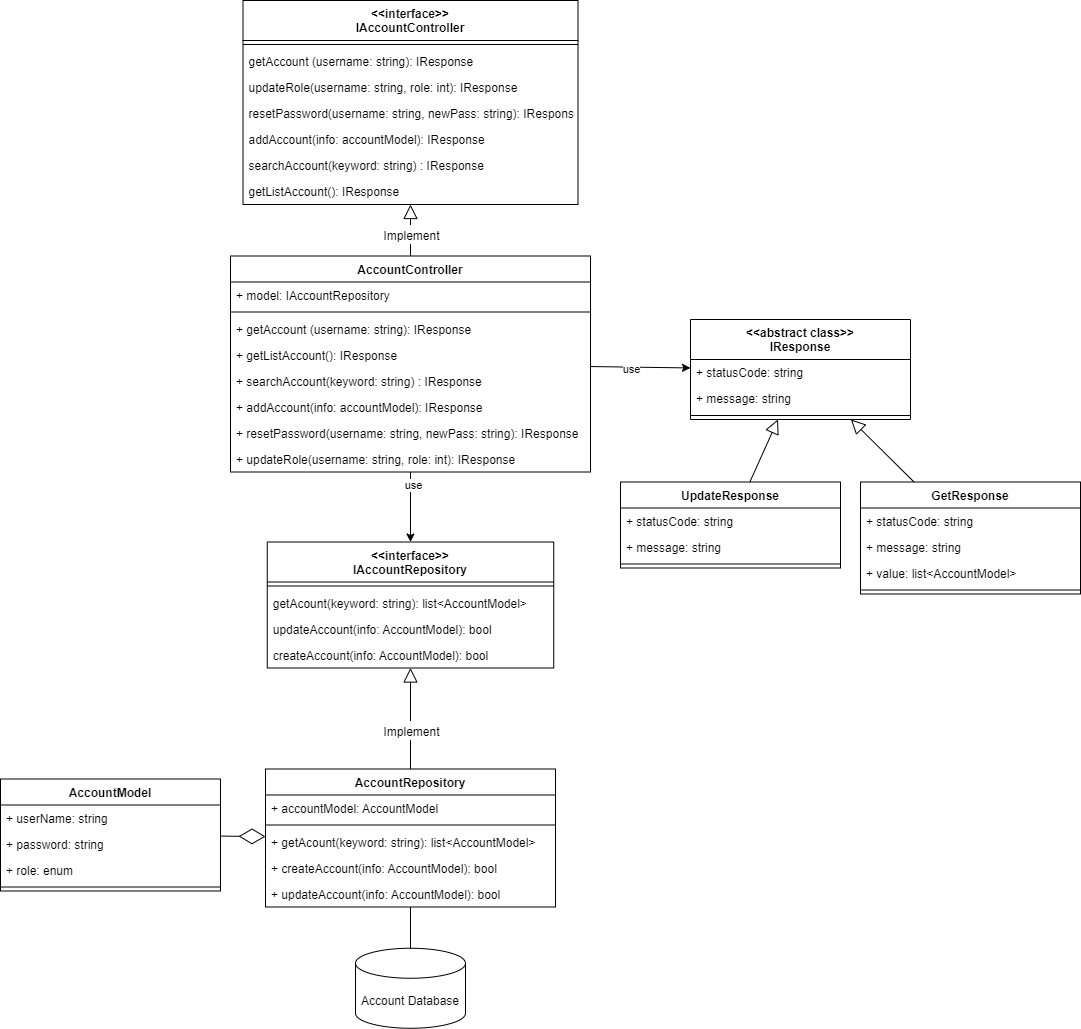
\includegraphics[width=11cm]{img/Architecture/service/AccountService.png}
	\newline
	\caption{Lược đồ class của Account Service}
\end{figure}



\subsubsection{Staff Service}
\begin{figure}[!htp]
	\centering
	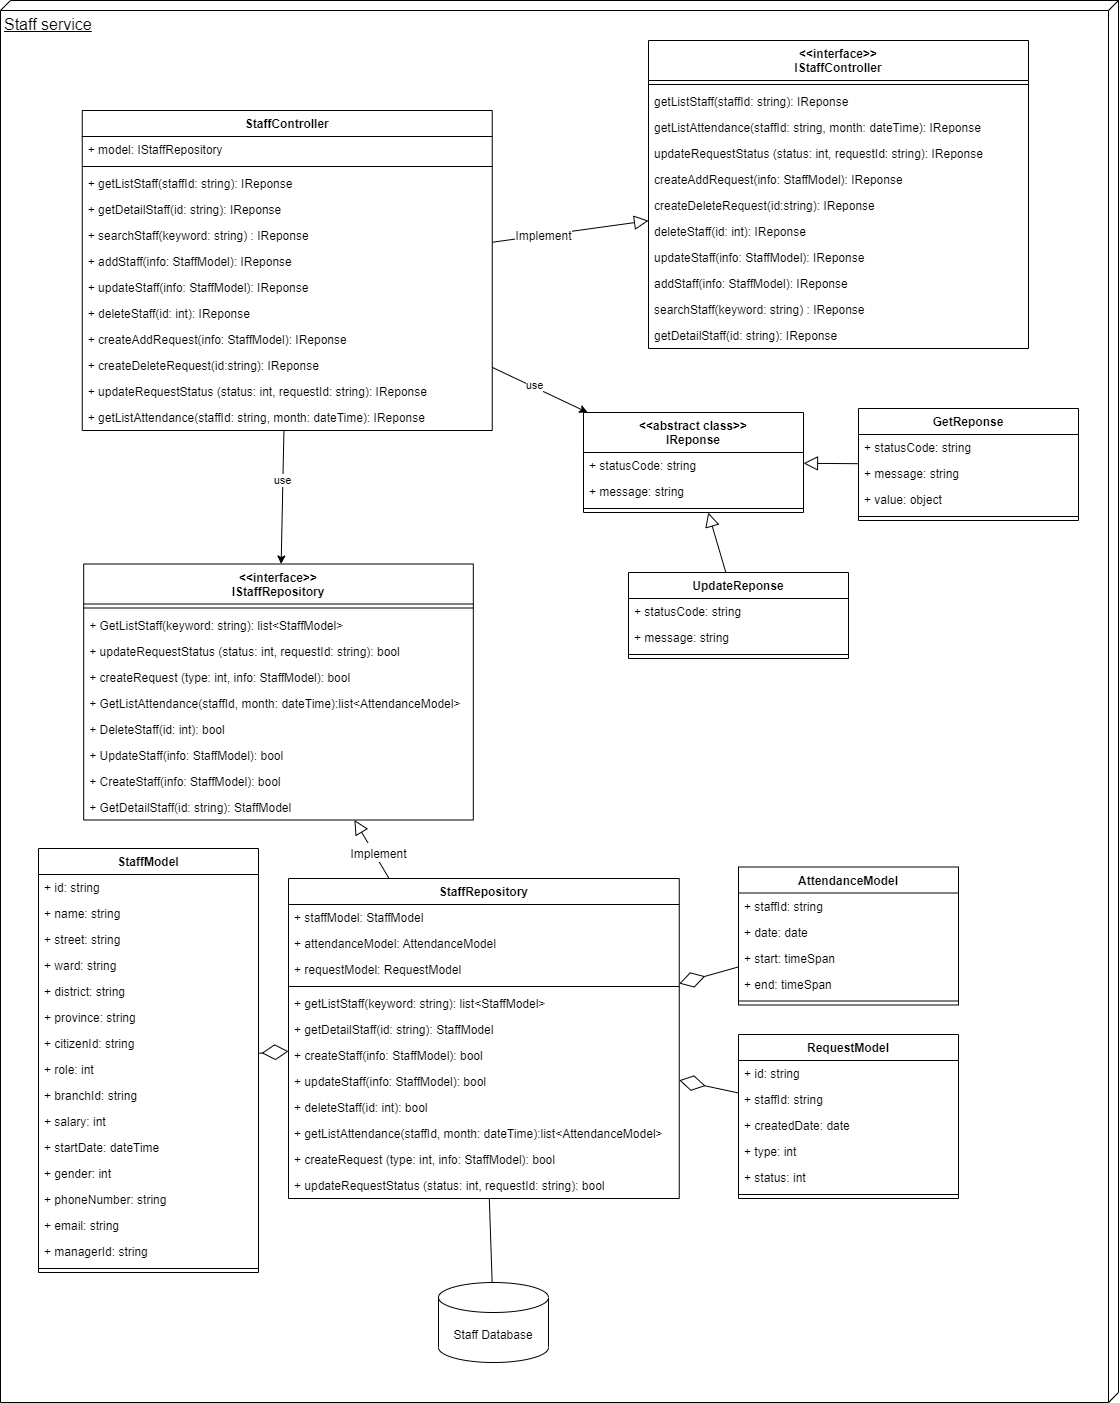
\includegraphics[width=11cm]{img/Architecture/service/StaffService.png}
	\newline
	\caption{Lược đồ class của Staff Service}
\end{figure}

\subsubsubsection*{StaffRepository}
Thuộc tính:
\begin{itemize}
	\item staffModel: Chứa đối tượng StaffModel
	\item attendanceModel: Chứa đối tượng AttendanceModel
	\item requestModel: Chứa đối tượng RequestModel
\end{itemize}
Phương thức:
\begin{itemize}
	\item getListStaff(keyword: string): Lấy danh sách nhân viên theo từ khóa
	\item getDetailStaff(id: string): Lấy thông tin chi tiết một nhân viên
	\item createStaff(info: StaffModel): Thêm một nhân viên mới
	\item updateStaff(info: StaffModel): Cập nhật thông tin một nhân viên
	\item deleteStaff(id: string): Xóa một nhân viên
	\item getListAttendance(staffId, month: dateTime): Lấy danh sách điểm danh của nhân viên
	\item createRequest (type: int, info: StaffModel): Tạo một yêu cầu về thêm, xóa nhân viên
	\item updateRequestStatus (status: int, requestId: string): Cập nhật trạng thái cùa yêu cầu
\end{itemize}

\subsubsubsection*{StaffModel}
Thuộc tính:
\begin{itemize}
	\item id: Id của nhân viên
	\item name: Tên của nhân viên
	\item requestModel: Chứa đối tượng RequestModel
	\item street: Tên đường của nhân viên
	\item ward: Phường của nhân viên
	\item distric: Quận của nhân viên
	\item province: Tỉnh của nhân viên
	\item citizenId: Căn cước của nhân viên
	\item role: Vị trí của nhân viên
	\item branchId: Id nơi làm việc của nhân viên
	\item salary: Mức lương của nhân viên
	\item startDate: Ngày bắt đầu làm việc của nhân viên
	\item endDate: Ngày kết thúc làm việc của nhân viên
	\item gender: Giới tính của nhân viên
	\item phoneNumber: Số điện thoại của nhân viên
	\item email: Email của nhân viên
\end{itemize}


\subsubsubsubsection*{AttendaceModel}
Thuộc tính:
\begin{itemize}
	\item staffId: Id của nhân viên
	\item date: Ngày làm việc
	\item start: Thời gian bắt đầu
	\item end: Thờ gian kết thúc
\end{itemize}

\subsubsubsubsection*{RequestModel}
Thuộc tính:
\begin{itemize}
	\item id: Id của yêu cầu
	\item staffId: Id của nhân viên
	\item createDate: Ngày tạo
	\item type: Loại yêu cầu
	\item status: Trạng thái yêu cầu
\end{itemize}

\subsubsubsubsection*{StaffController}
Thuộc tính:
\begin{itemize}
	\item repo: Chứa đối tượng StaffRepository
\end{itemize}
Phương thức:
\begin{itemize}
	\item getListStaff(branchId: string): Lấy danh sách nhân viên theo chi nhánh
	\item getDetailStaff(id: string): Lấy thông tin chi tiết một nhân viên
	\item searchStaff(keyword: string): Lấy danh sách nhân viên theo từ khóa
	\item createStaff(info: StaffModel): Thêm một nhân viên mới
	\item updateStaff(info: StaffModel): Cập nhật thông tin một nhân viên
	\item deleteStaff(id: string): Xóa một nhân viên
	\item createAddRequest(info: StaffModel): Tạo một yêu cầu thêm nhân viên
	\item createDeleteRequest(id:string): Tạo một yêu cầu về xóa nhân viên
	\item updateRequestStatus (status: int, requestId: string): Cập nhật trạng thái cùa yêu cầu
	\item getListAttendance(staffId, month: dateTime): Lấy danh sách điểm danh của nhân viên
\end{itemize}

\subsubsubsubsection*{UpdateResponse - GetResponse}
Thuộc tính:
\begin{itemize}
	\item statusCode: Mã trạng thái của phản hồi
	\item message: Thông điệp của phản hồi
	\item value: Các dữ liệu trả về đối với các yêu cầu HTTP GET
\end{itemize}





\subsubsection{Branch Service}
\begin{figure}[!htp]
	\centering
	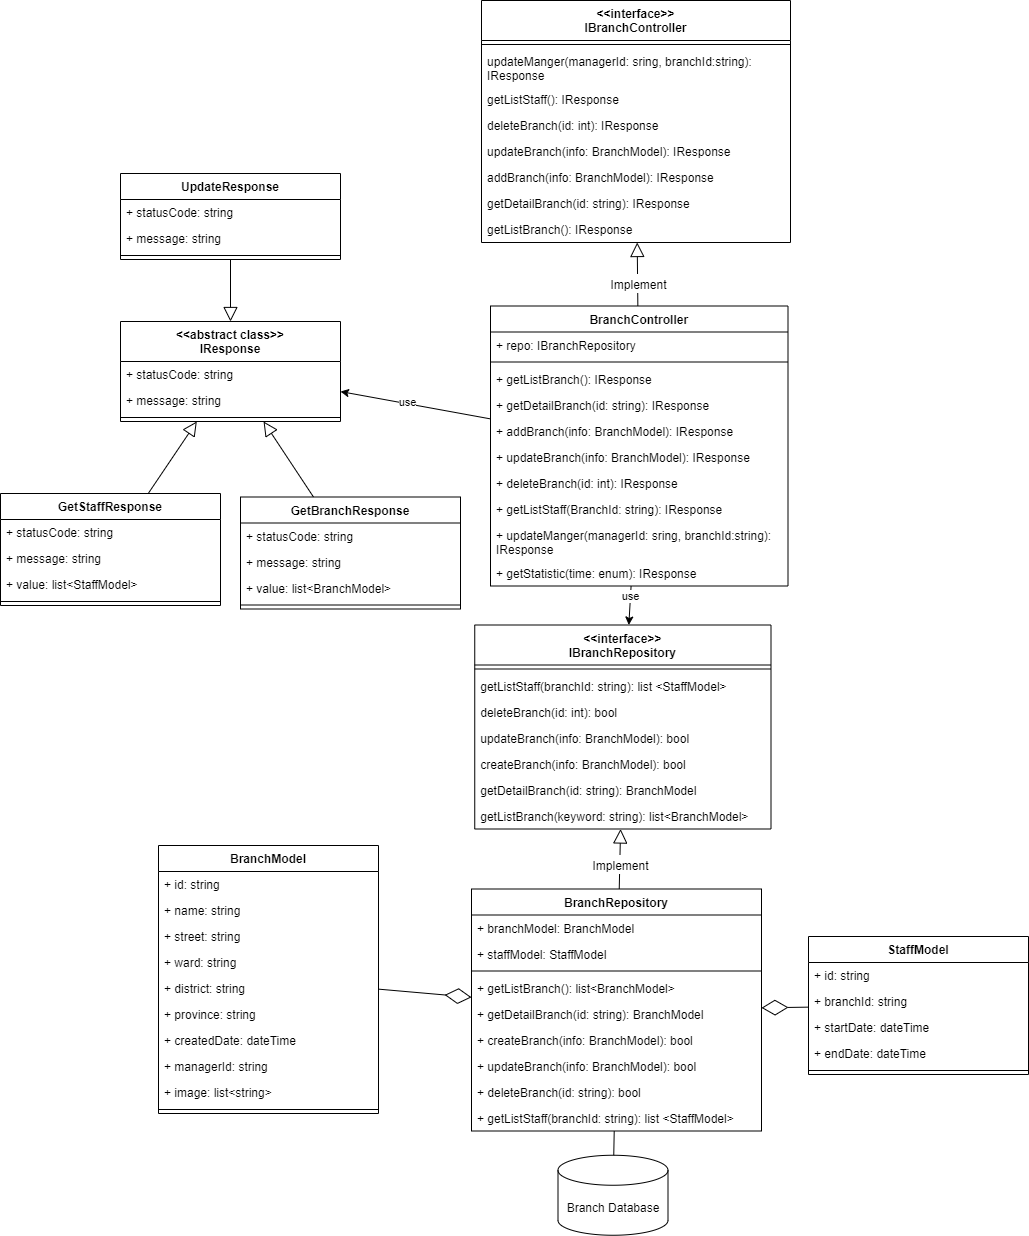
\includegraphics[width=10cm]{img/Architecture/service/BranchService.png}
	\newline
	\caption{Lược đồ class của Branch Service}
\end{figure}

\subsubsubsubsection*{BranchRepository}
Thuộc tính:
\begin{itemize}
	\item branchModel: Chứa đối tượng BranchModel
	\item staffModel: Chứa đối tượng StaffModel
\end{itemize}
Phương thức:
\begin{itemize}
	\item getListBranch(): Lấy danh sách chi nhánh
	\item getDetailBranch(id: string): Lấy thông tin chi tiết một chi nhánh
	\item createBranch(info: BranchModel): Thêm một chi nhánh mới
	\item updateBranch(info: BranchModel): Cập nhật thông tin một chi nhánh
	\item deleteBranch(id: string): Xóa một chi nhánh
	\item getListStaff(BranchId: string): Lấy danh sách nhân viên của chi nhánh
\end{itemize}

\subsubsubsubsection*{BranchModel}
Thuộc tính:
\begin{itemize}
	\item id: Id của chi nhánh
	\item name: Tên của chi nhánh
	\item street: Tên đường của chi nhánh
	\item ward: Phường của chi nhánh
	\item distric: Quận của chi nhánh
	\item province: Tỉnh của chi nhánh
	\item createdDate: Ngày tạo chi nhánh
	\item managerId: Id của người quản lý
	\item image: Các hình ảnh của chi nhánh
\end{itemize}

\subsubsubsubsection*{StaffModel}
Thuộc tính:
\begin{itemize}
	\item id: Id của nhân viên
	\item branchId: Id của chi nhánh làm việc
	\item startDate: Thời gian bắt đầu làm việc tại chi nhánh
	\item endDate: Thời gian kết thúc làm việc tại chi nhánh
\end{itemize}

\subsubsubsubsection*{BranchController}
Thuộc tính:
\begin{itemize}
	\item repo: Chứa đối tượng repository
\end{itemize}
Phương thức:
\begin{itemize}
	\item getListBranch(): Lấy danh sách chi nhánh
	\item getDetailBranch(id: string): Lấy thông tin chi tiết một chi nhánh
	\item addBranch(info: BranchModel): Thêm một chi nhánh mới
	\item updateBranch(info: BranchModel): Cập nhật thông tin một chi nhánh
	\item deleteBranch(id: int): Xóa một chi nhánh
	\item getListStaff(BranchId: string): Lấy danh sách nhân viên của chi nhánh
	\item updateManger(managerId: sring, branchId:string): Cập nhật quản lý chi nhánh
	\item getStatistic(time: enum): Lấy thông tin thống kê lợi nhuận, doanh thu.
\end{itemize}

\subsubsubsubsection*{UpdateResponse - GetStaffResponse - GetBranchResponse }
Thuộc tính:
\begin{itemize}
	\item statusCode: Mã trạng thái của phản hồi
	\item message: Thông điệp của phản hồi
	\item value: Các dữ liệu trả về đối với các yêu cầu HTTP GET
\end{itemize}



\subsubsection{Event Service}
\begin{figure}[!htp]
	\centering
	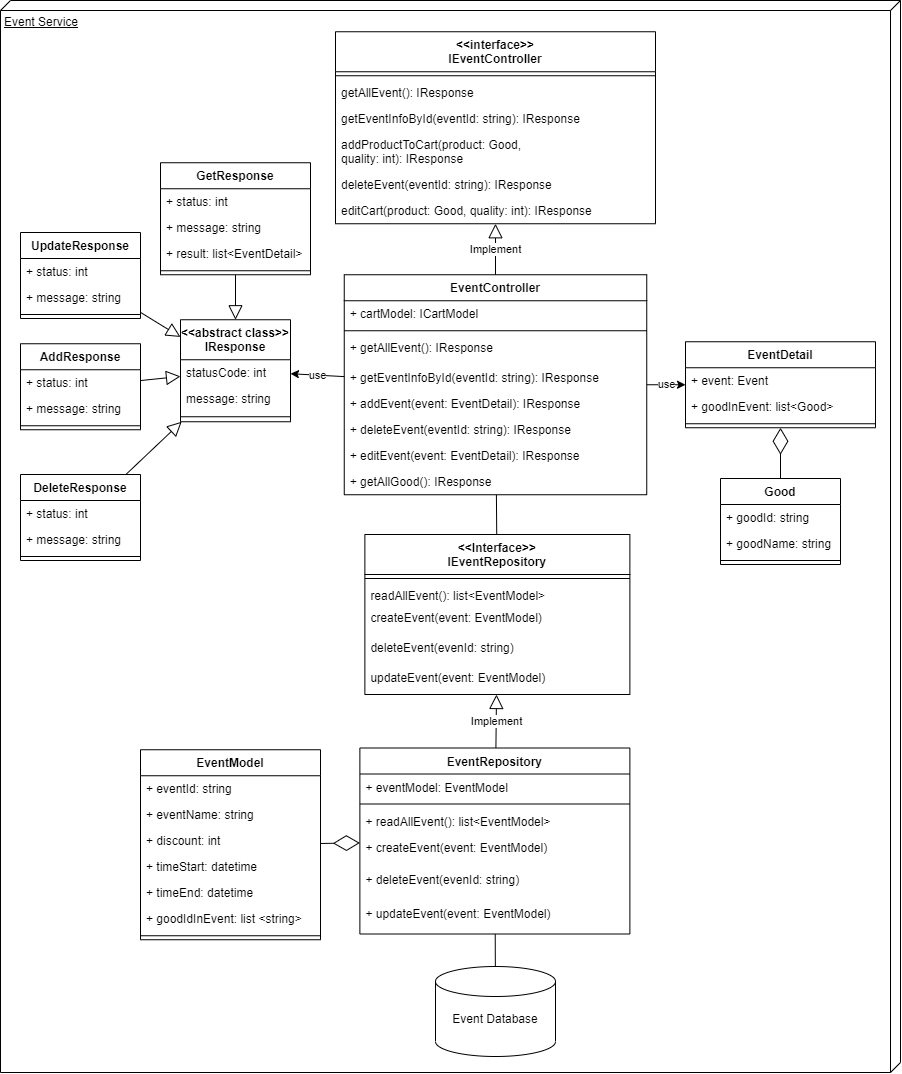
\includegraphics[width=11cm]{img/Architecture/service/EventService.png}
	\newline
	\caption{Lược đồ class của Event Service}
\end{figure}


\subsubsection{Warehouse Service}
\begin{figure}[!htp]
	\centering
	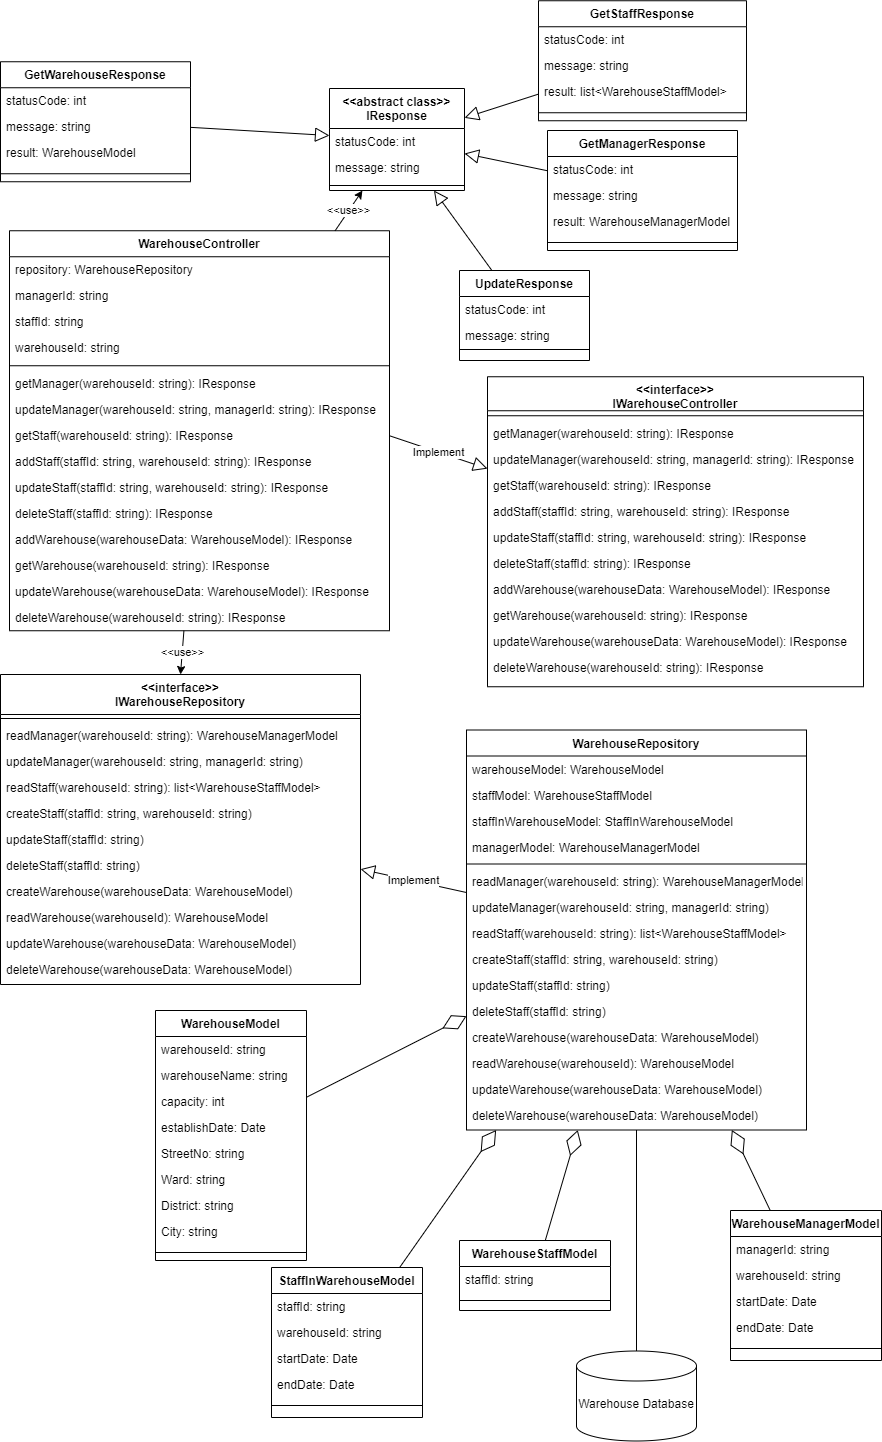
\includegraphics[width=11cm]{img/Architecture/service/WarehouseService.png}
	\newline
	\caption{Lược đồ class của Warehouse Service}
\end{figure}


\subsubsection{Statistic Service}
\begin{figure}[!htp]
	\centering
	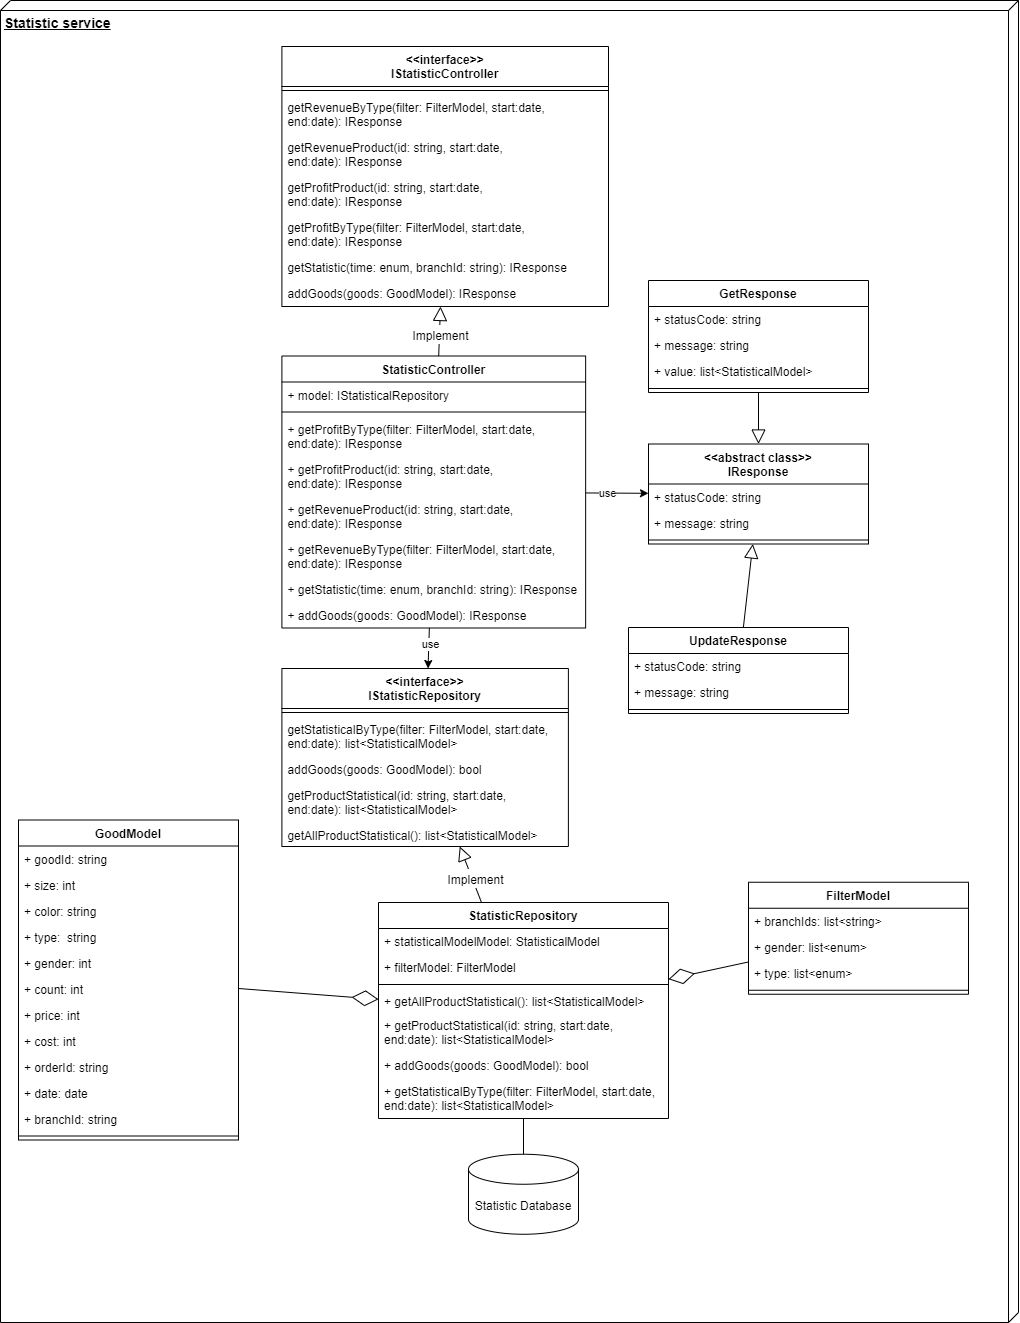
\includegraphics[width=11cm]{img/Architecture/service/StatisticService.png}
	\newline
	\caption{Lược đồ class của Statistic Service}
\end{figure}
\textbf{Mô tả:}
\begin{quote}
	\begin{itemize}
		\item ...
		\item ...
	\end{itemize}
\end{quote}

\subsubsection{Goods Service}
\begin{figure}[!htp]
	\centering
	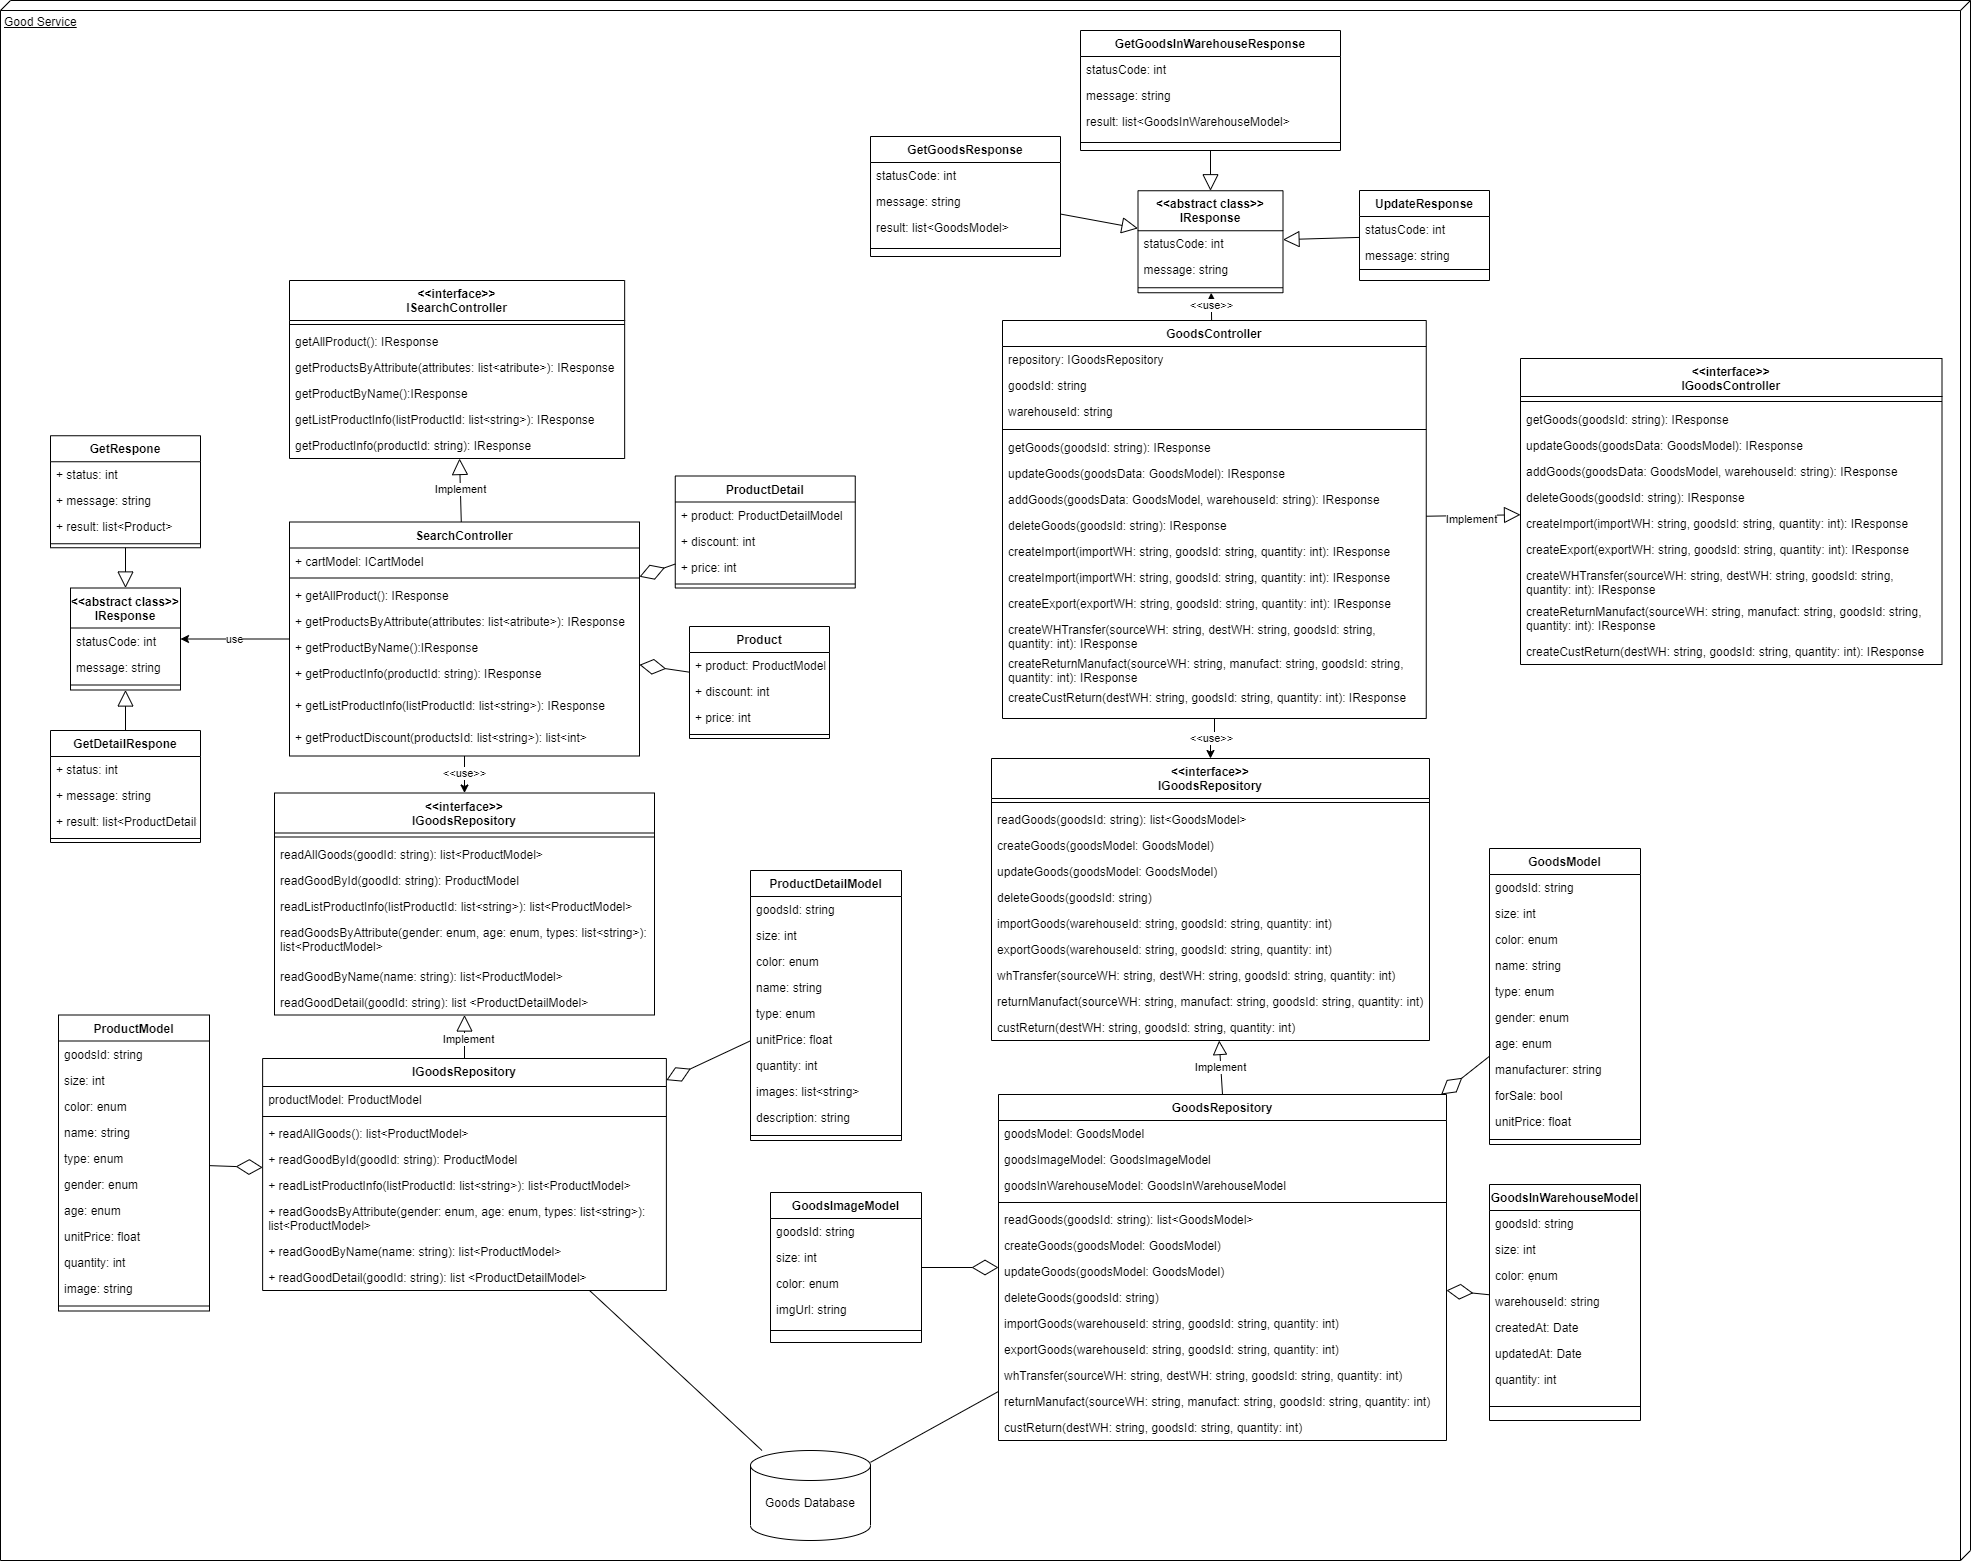
\includegraphics[width=17cm]{img/Architecture/service/GoodsService.png}
	\newline
	\caption{Lược đồ class của Goods Service}
\end{figure}

